\documentclass{article}
\usepackage[utf8]{inputenc}
\usepackage{amsmath}
\usepackage{chngcntr}
\usepackage[english]{babel}
\usepackage[autostyle, english = american]{csquotes}
\usepackage{graphicx}
\usepackage{mathtools}
\usepackage{listings}
\usepackage{xcolor}
\usepackage{float}

%Includes "References" in the table of contents
\usepackage[nottoc]{tocbibind}

\MakeOuterQuote{"}
\renewcommand{\theequation}{\arabic{section}.\arabic{equation}}
\DeclarePairedDelimiter\ceil{\lceil}{\rceil}
\DeclarePairedDelimiter\floor{\lfloor}{\rfloor}

\counterwithin*{equation}{section}

% make listings look nice with line-wrapping
\lstset{ %Formatting for code in appendix
    basicstyle=\footnotesize,
    numbers=left,
    stepnumber=1,
    tabsize=1,
    frame=single,
    breaklines=true,
    postbreak=\raisebox{0ex}[0ex][0ex]{\ensuremath{\color{red}\hookrightarrow\space}}
}

\setlength{\parindent}{0em} % Don't indendent paragraphs
\setlength{\parskip}{1em} % Blank line between paragraphs

\title{ECS 132 Final Project}
\author{Joseph Lewis, Aaron Kaloti, Sean Malloy}
\date{due: Friday, March 24, 2017, 11:59pm}

\begin{document}
\maketitle

\tableofcontents  % Just this one line does table of contents :D

\newpage
\section{Image Processing}

\subsection{getnonbound(imgobj)}

It was expected that the \textbf{getnonbound} function written to organize the data from an image into a format viable for operating on image smoothing and noise reduction would have a very long runtime.  This could be expected, from the nature of the function - it has to store each of the grayscale data points in the image into a vector, whose length will be the number of pixels in the image (minus the border pixels) and also store each neighboring pixel value into a matrix of the same length, with four times the number of total entries.

If approached naively, the function could take many minutes to run for even one small file.  For large files or many numbers of files, it could take even longer - a dramatic issue if this denoising regression is to be applied to many images by the same user.  But, by avoiding R loops, which have additional overhead due to the nature of R as an interpreted language, and instead using vectorization, the function does not need to run slowly.

Our resulting function, as provided in the appendix, runs with no noticeable lag for the sample image provided, and quite quickly (in a matter of no more than a few seconds per image) for large (HD: 1920 x 1080) images (also provided in the appendix).  We describe exactly how we got the function running faster in the code discussion in the appendix.  We feel that this running time is acceptable for the process, as even with large images the user has no significant waiting period for the function to finish. 

\subsection{Regressing on Neighboring Pixels}

The estimated prediction function from regressing $y$ on $x$ as run through the \textbf{getnonbound(imgobj)} function are given in the equation below:
\begin{equation}
y = -0.007 + 0.15183 \cdot N + 0.15107 \cdot S + 0.35867 \cdot E + 0.35866 \cdot W
\end{equation}
We see that for this image, two significant trends emerge based on the coefficients.  The first trend is that the neighboring east and west pixel grey-scale values contribute more than twice as much to the prediction of the center value than the north and south neighbors do.  We can expect this from the nature of the \textit{LaLa Land} picture: it is landscape, so it has many more horizontal pixels than vertical ones; and its color patterns show clearly in horizontal stripes, aided by the coloration of the sky across the top and the road through the bottom.  We can use the sizing of the image (768 x 433), having nearly twice as many horizontal pixels as vertical ones, to explain the majority of this difference.  But, we notice that the image size is not more than twice as wide as it is tall, so the extra emphasis from the horizontal pixels as predictors must come from the patterns within the image - the sky has distinct shades that hold in horizontal lines, the mountains provide a horizontal stripe of similar color, etc.  These patterns help skew the image towards favoring horizontal neighboring predictors.

The second trend is that the north and south pixels have nearly the same coefficients as a pair, and the east and west pixels also have nearly the same coefficients.  This makes sense - that the pixels in an image both above and below the target pixel will have an equal effect on that pixel's predicted value, and the pixels in an image both right and left of the target pixel will also have an equal effect on that pixel's predicted value.

\subsection{Image Smoothing}

We were inspired in the following analysis by an article written by Robert Fisher, Simon Perkins, Ashley Walker and Erik Wolfart \cite{mean-filter}.

In typical image smoothing, we would use a 'kernel' to predict the pixel values.  A kernel is just a size and a shape within which to look at additional pixels surrounding some center one.  In our case, we used a plus shaped kernel that looked at only the orthogonally adjacent neighbors to an interior pixel in the image, and used standard linear regression techniques to examine how well those four neighboring pixels - north, south, east, and west - predicted their center.

A standard kernel to use in image smoothing is a 3x3 square centered on the interested pixel.  This kernel takes the average values among \textit{all} 9 pixels in the square (including the center), weighting them equally, and uses that average to predict the value for the center pixel, and replace it.  The result is an image that has smoothed lines and can be somewhat blurred, but reduces any noise in the image.  

However, it can be difficult to remove uniform (0,1) noise across an image.  This type of noise is usually referred to as 'salt and pepper' noise, as it looks like white, grey, and black specks sprinkled across the image's surface.  In typical average-based image smoothing, the averages generated about a noisy pixel can be significantly changed by the pixel itself being so far from the values around it.  It skews the average and the resulting smoothing only adjusts the noisy sections of image so much, leaving a blurred and still speckled image.

In our image-smoothing algorithm, we will apply our plus shaped kernel, which does not include the center pixel, to each interior pixel in a 'salt and pepper' noisy image.  By using a linear regression model (essentially, a weighted-average smoothing model, with the weights determined by the linear regression coefficients) which allows the patterns in the image and the image's size to influence the strength of any neighboring pixel's influence on the center pixel in each kernel, we reduce the effect of noise further than simple average-based image smoothing, but not entirely.  However, we also run the risk of noise on a horizontal scale having greater effect than noise on a vertical one.

\subsection{Three Image Smoothing Examples}

Now we example the regression-based smoothing on the following three images and discuss its merits.  We first had to apply random 'salt and pepper' noise to these images.  Finding the proper amount of noise to add was a matter of trial and error, and the function we used to apply the noise can be seen and is analyzed in the appendix.  We settled on  populating one percent of the pixels (0.01 proportionately) with random noise, as it was easily apparent that noise had corrupted the image, but not so noisy that the original image could not be made out or that the denoise function would be ineffective. Then we applied our regression in an attempt to remove the noise.

\subsection{Example 1 - LaLa Land}

\begin{figure}[H]
    \begin{center}
        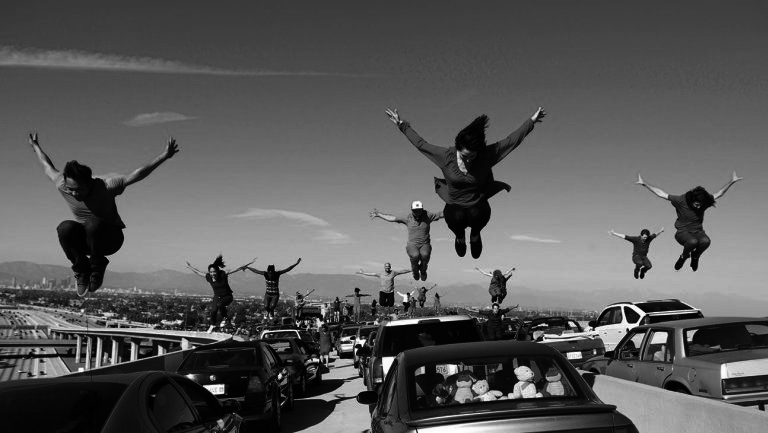
\includegraphics[width=0.75\textwidth]{LLL.jpg}
    \end{center}
  \caption{The original image.}
\end{figure}

\begin{figure}[H]
    \begin{center}
        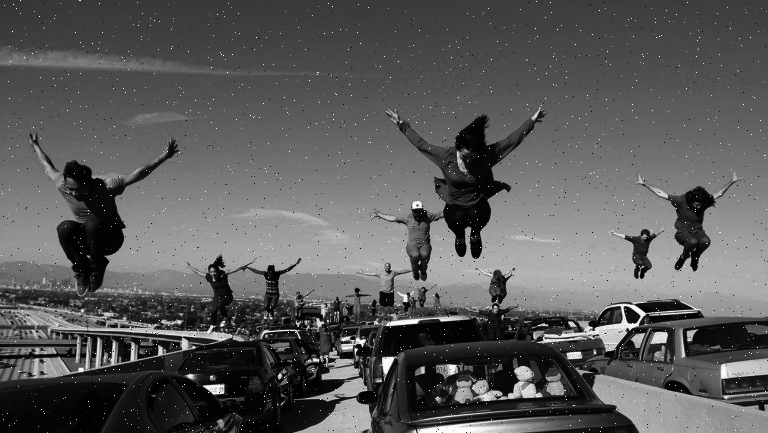
\includegraphics[width=0.75\textwidth]{noised_LLL.jpg}
    \end{center}
  \caption{The image with U(0,1) random noise.}
\end{figure}

\begin{figure}[H]
    \begin{center}
        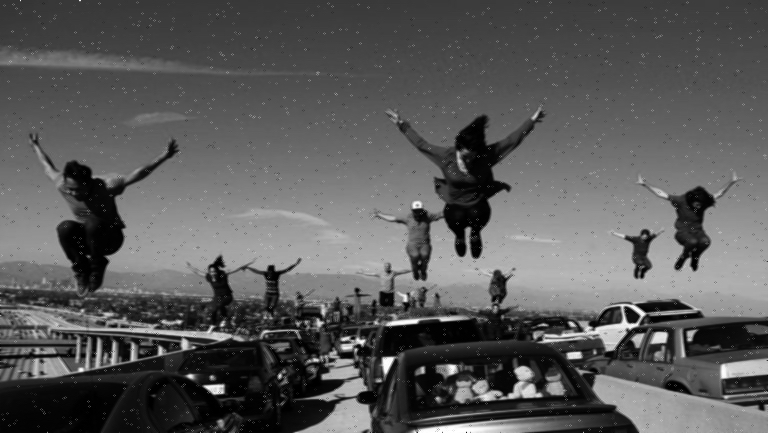
\includegraphics[width=0.75\textwidth]{denoised_LLL.jpg}
    \end{center}
  \caption{After the denoising algorithm is applied.}
\end{figure}

Notice that for this small of an image, the denoise function can only do so much.  The patterns which are apparent horizontally do help reduce any vertical noise, but we can still see the 'salt and pepper' noise and the image lines looked blurred.  To the smoothing algorithm's credit, the image does look considerably less speckled when viewed from a distance than its noisy counterpart.

The regression function for the original image is given in equation (2.1).  The regression function for the noisy image shown above is:
\begin{equation}
y = -0.004 + 0.18614 * N + 0.18567 * S + 0.31975 * E + 0.31971 * W
\end{equation}
We can see that the impact of the noise is to reduce the horizontal patterns in the image effect on the regression coefficients, but not by much.  It is the nature of the type of noise that still makes the de-noised image not appear very "fixed".

\subsection{Example 2 - Dungeons and Dragons Image (High Resolution)}

\begin{figure}[H]
    \begin{center}
        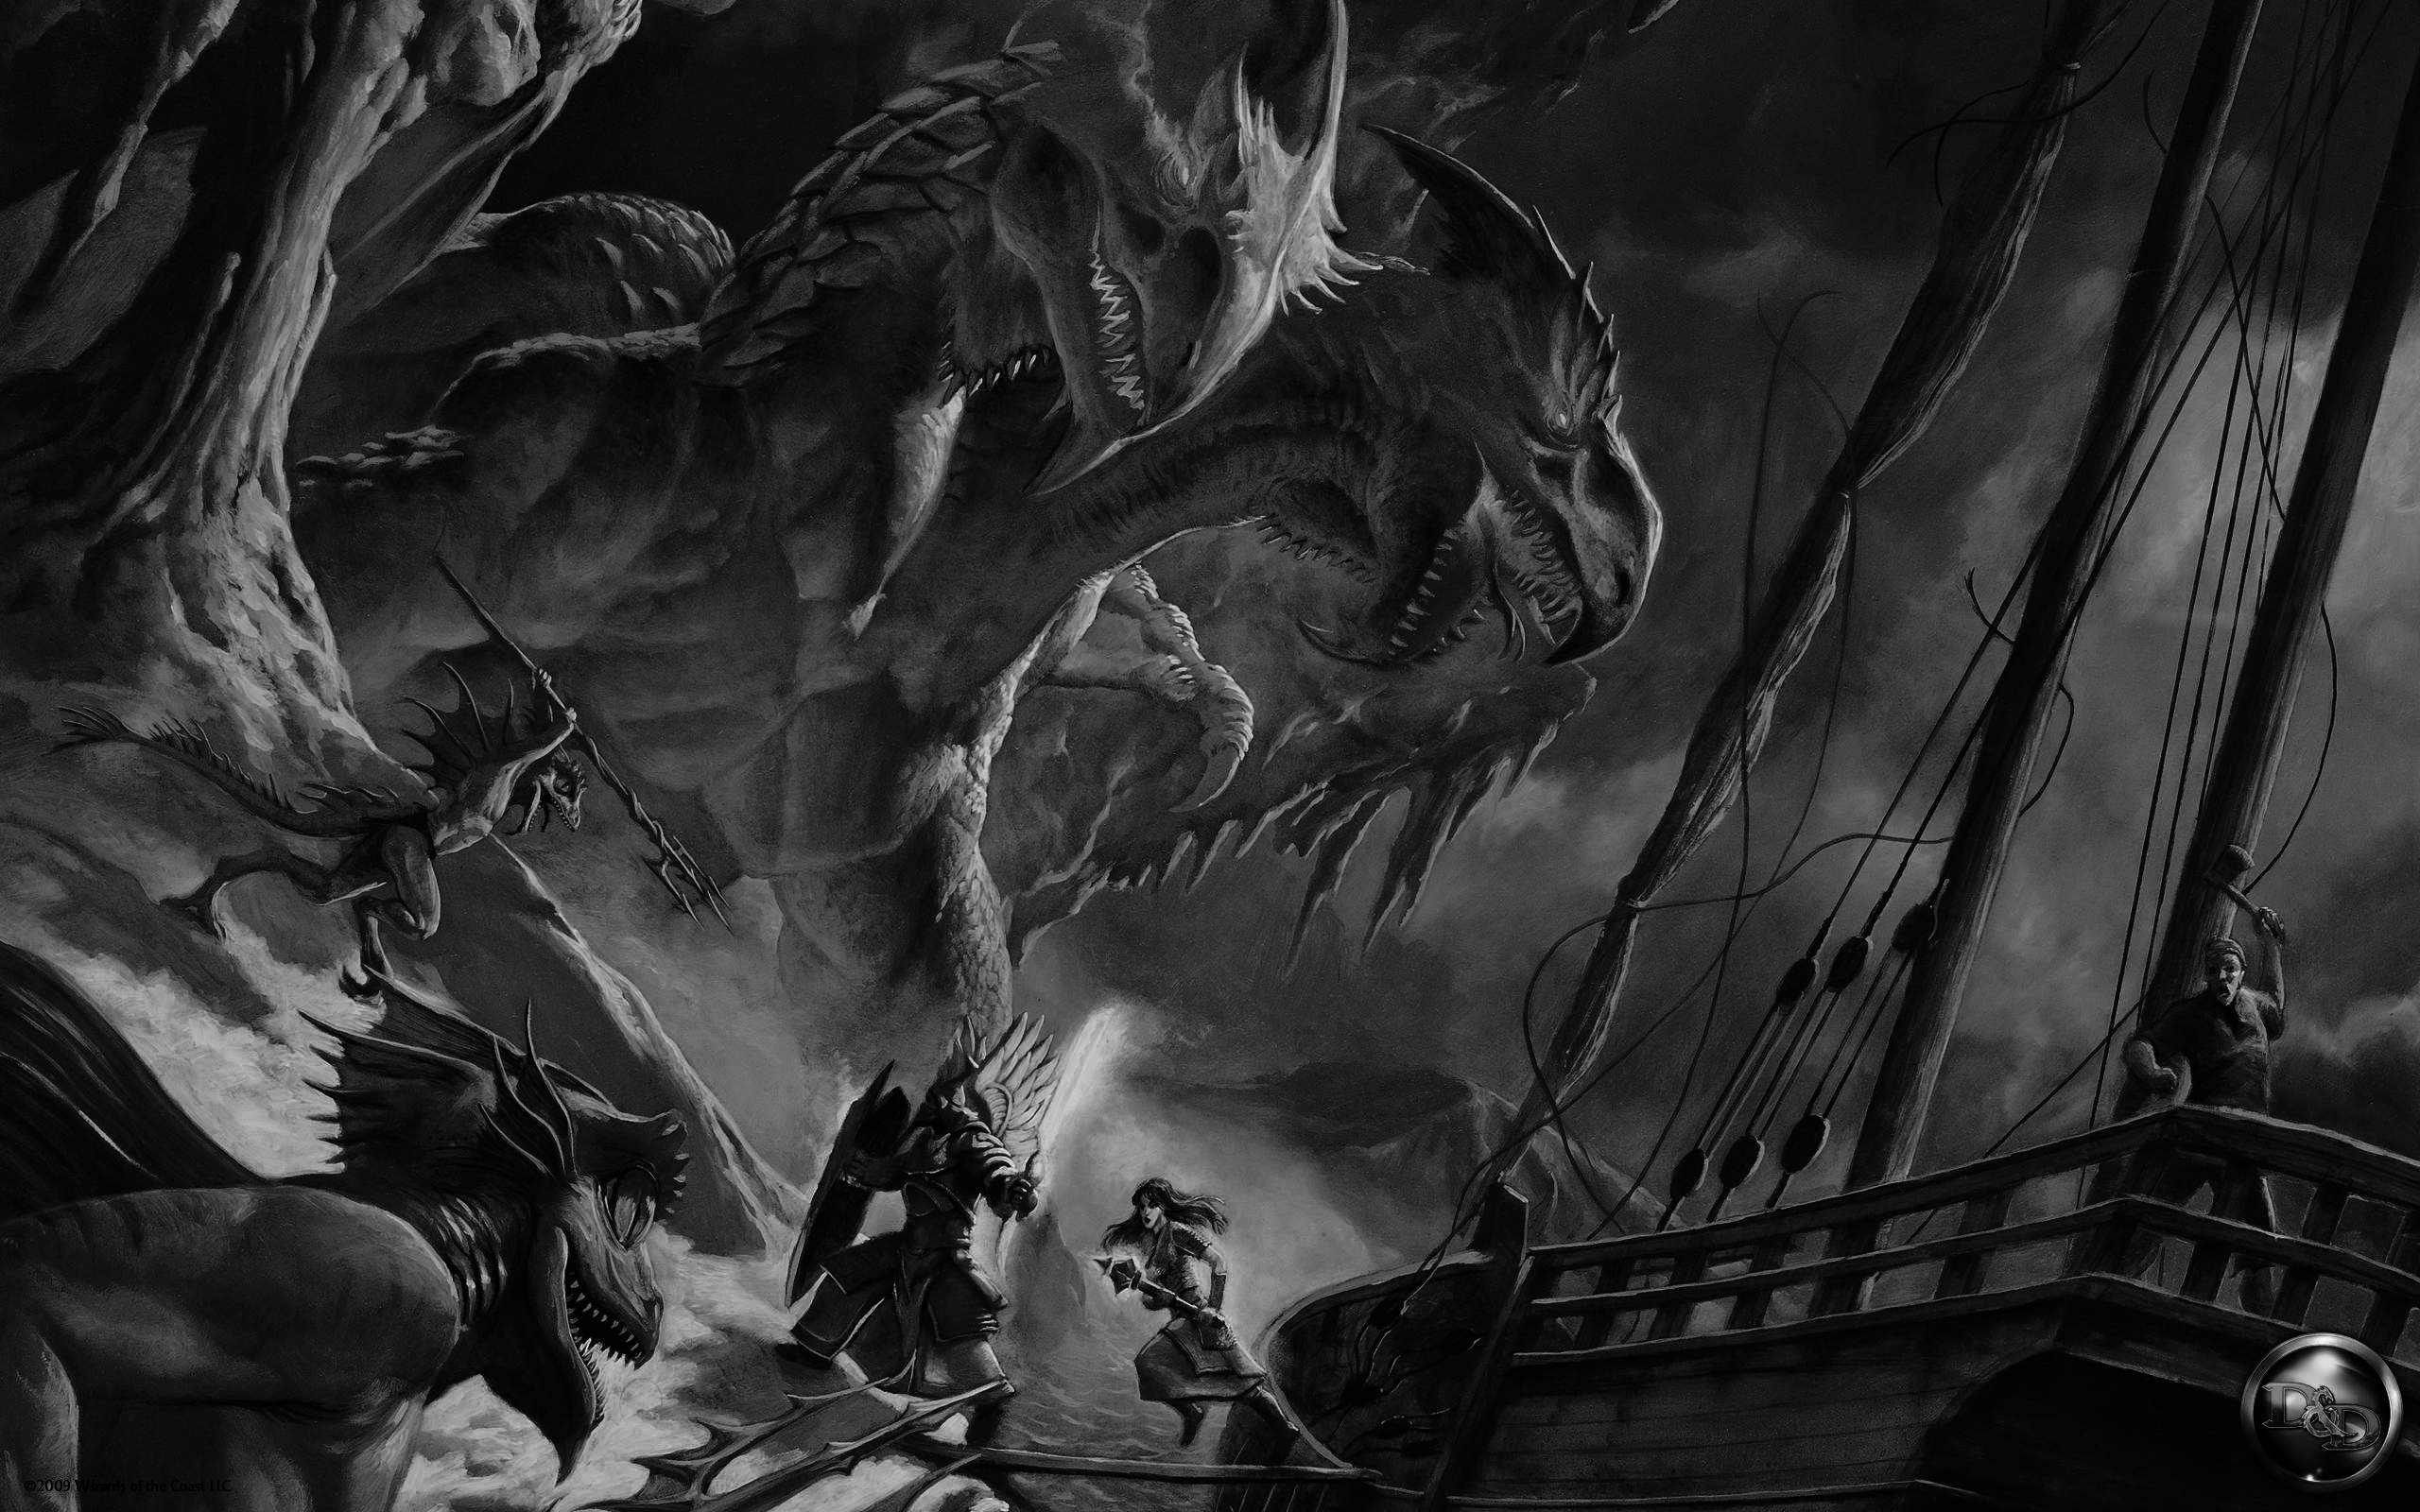
\includegraphics[width=0.75\textwidth]{dragon.jpg}
    \end{center}
  \caption{The original image.}
\end{figure}

\begin{figure}[H]
    \begin{center}
        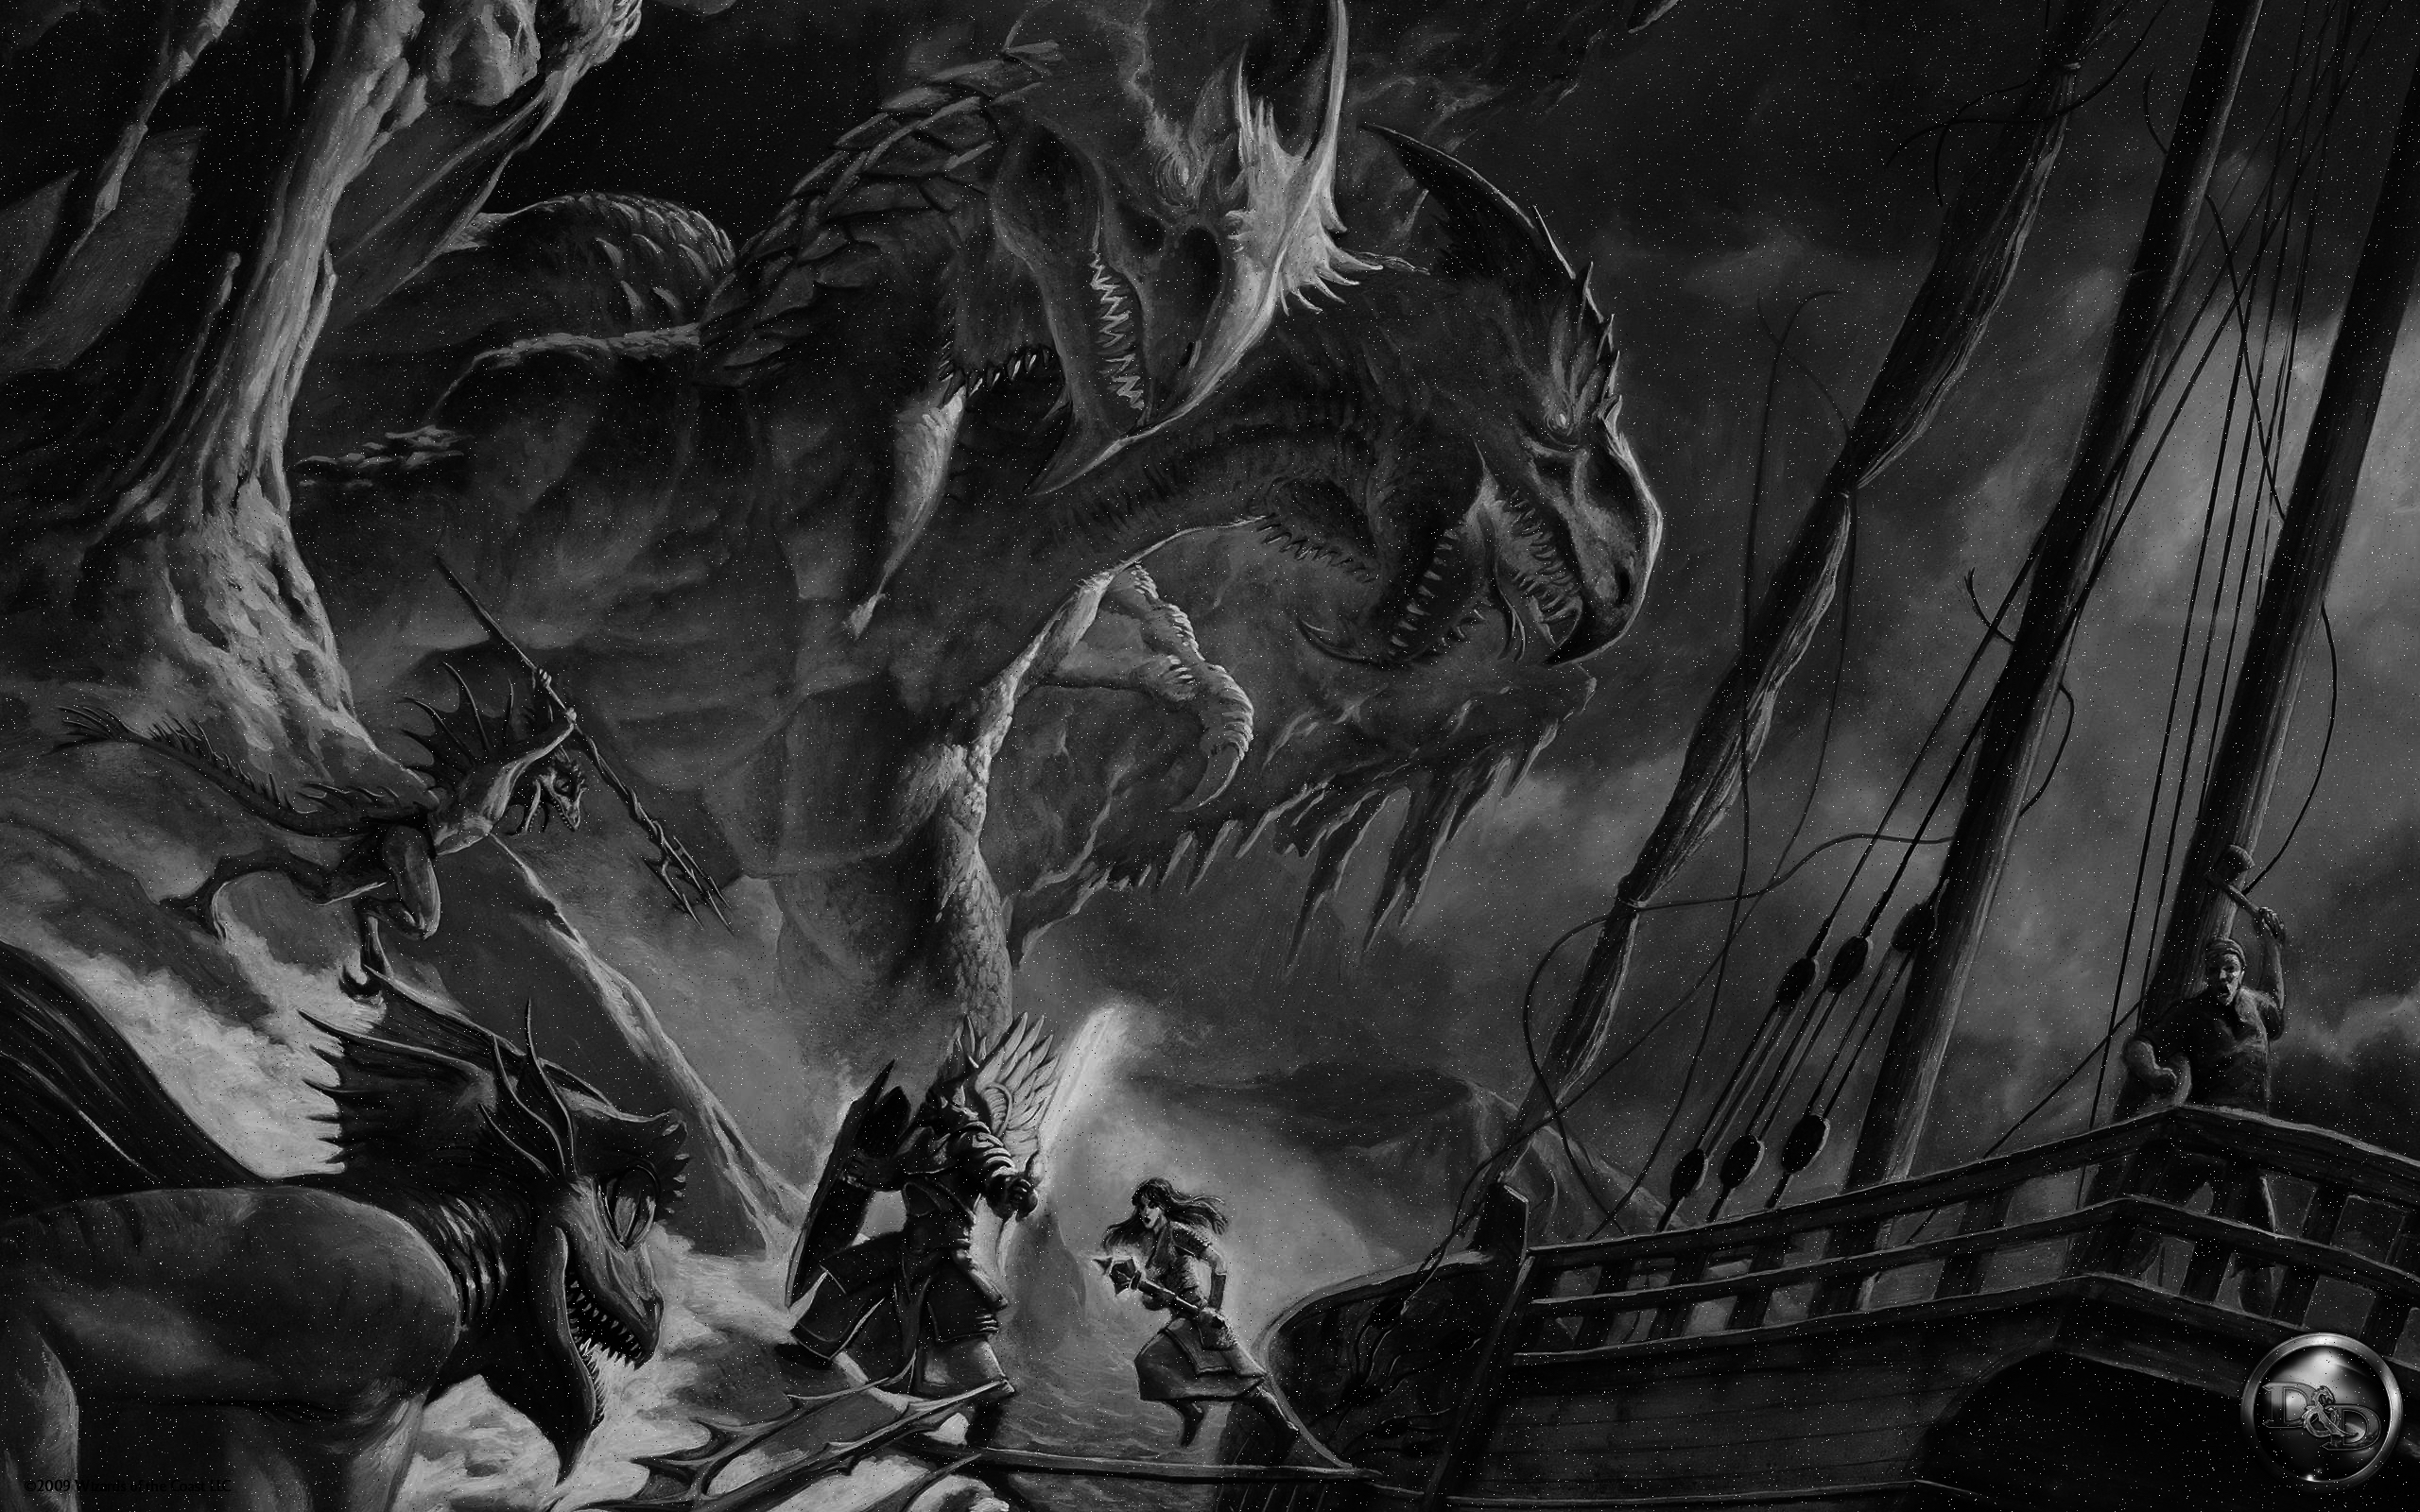
\includegraphics[width=0.75\textwidth]{noised_dragon.jpg}
    \end{center}
  \caption{The image with U(0,1) random noise.}
\end{figure}

\begin{figure}[H]
    \begin{center}
        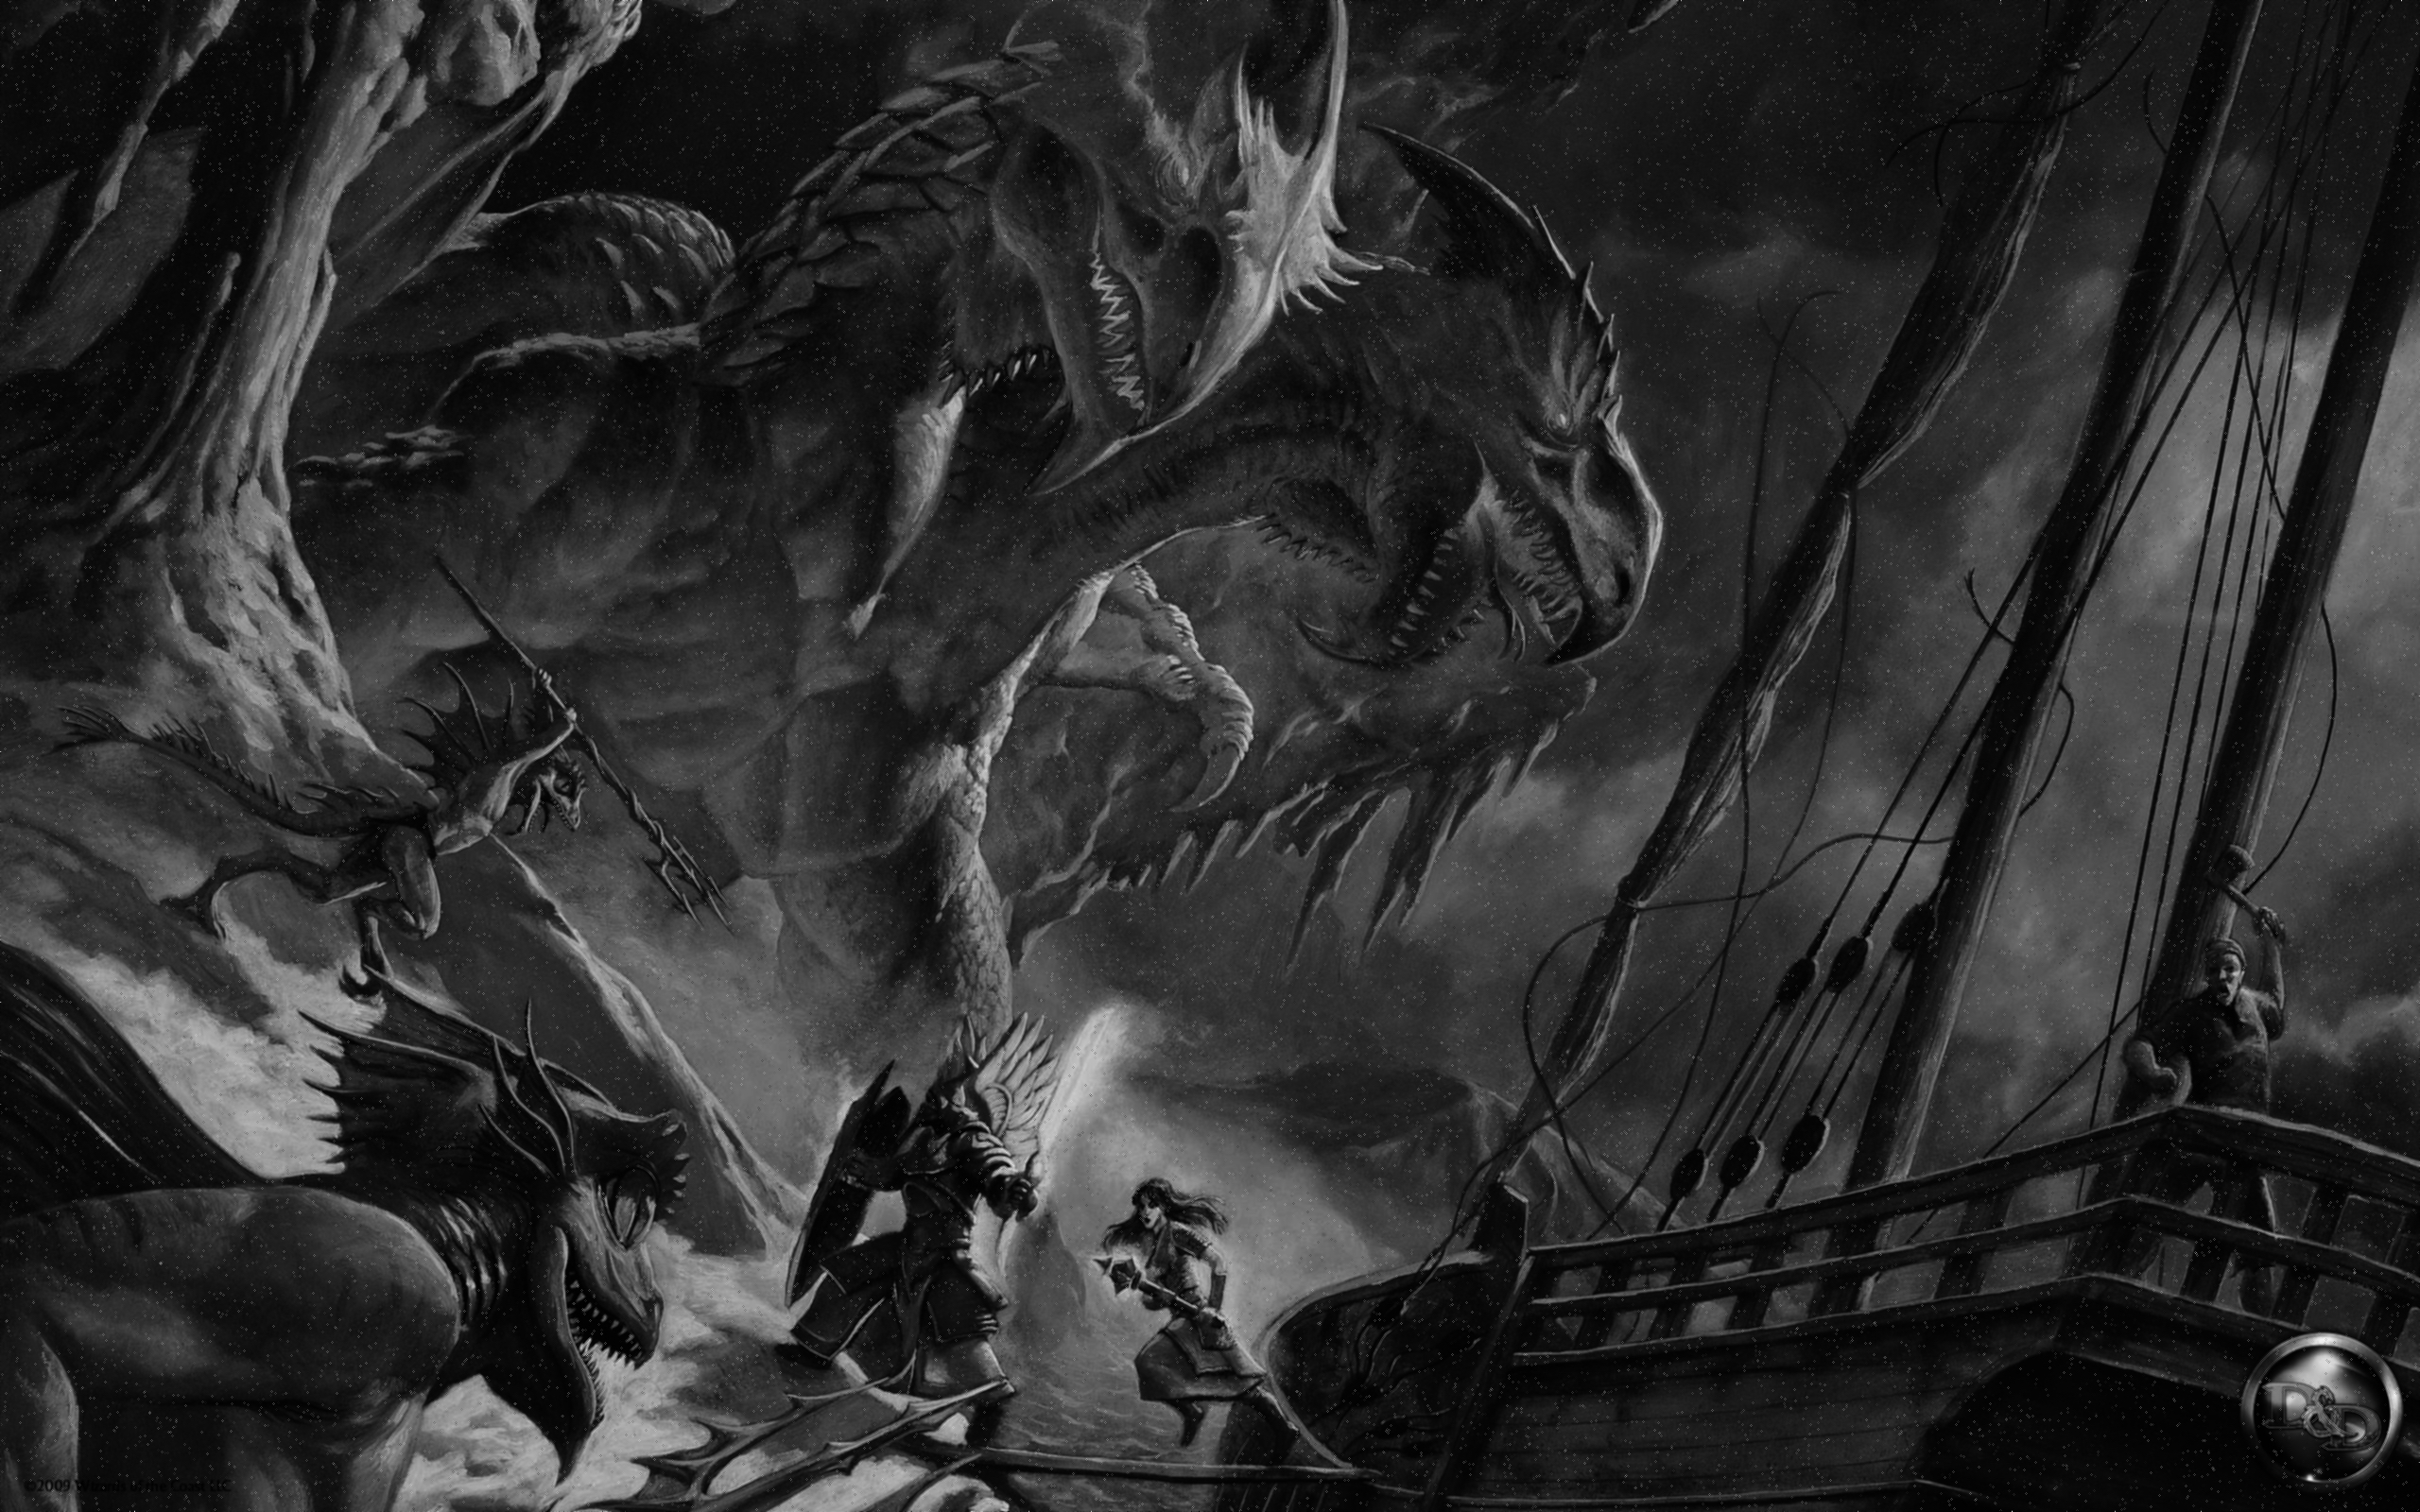
\includegraphics[width=0.75\textwidth]{denoised_dragon.jpg}
    \end{center}
  \caption{After the denoising algorithm is applied.}
\end{figure}

This image was selected because of its balance of black and white sections, as well as its high resolution.  The image provided the smoothest and cleanest result of all our test images after applying the regression-based smoothing.  We note that this likely stems from: the image's equal areas of light and dark patches, which cause the overall regression not to be skewed towards one side or the other; and primarily the image's size, which allow the smoothing algorithm to more accurately remove noise due to more accurate predictions (predicting based on much more data) and resolution scaling (our eyes can only perceive so much detail, so adding more pixels overall means that small alterations in a few pixels here and there are not as easily perceived).

The regression function for the original image is given by:
\begin{equation}
y = -0.00228 + 0.29579 \cdot N + 0.29549 \cdot S + 0.21076 \cdot E + 0.21075 \cdot W
\end{equation}
We see that despite the image's dimensions, the coefficients are larger for the north and south pixels than the east and west pixels.  This is because the image presents clear vertical patterns - the vertical masts, the coloring in the dragon's necks, and the rock pillar at the left.  This gives us an understanding that the more prominent factor for some images will be the patterns within the image, not the image dimensions.  This is especially true for larger images, where the number of pixels to regress on is so large that the patterns really have time to enforce themselves on the regression coefficients and even themselves out.

The regression function for the noisy image is given by:
\begin{equation}
y = 0.00261 + 0.25500 \cdot N + 0.25491 \cdot S + 0.23780 \cdot E + 0.23786 \cdot W
\end{equation}
We notice that this image presents a nearly even-average rounding method due to the addition of random noise.  Note that now the regression function is very nearly performing the same function as a simple average-based smoothing algorithm.  However, though the differences between the coefficients are small, giving each adjacent pixel nearly equal weight, it is significant that we are not just purely using averages.  The coefficients are the most optimized for this photo, and doing so for each photo results in the best looking de-noised images.  If we merely applied the equal-weight averages to every photo, it would not always have the cleanest looking result, because we would be weighting the contribution of certain pixels improperly.  We note that the noise applied to this photo was enough to skew the coefficients away from the patterns established and discussed in the previous paragraph.

\subsection{Example 3 - Blast from the Past}

\begin{figure}[H]
    \begin{center}
        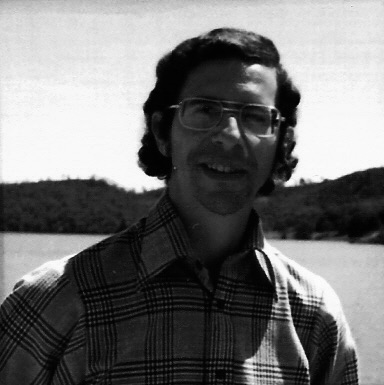
\includegraphics[width=0.5\textwidth]{matloff.jpg}
    \end{center}
  \caption{The original image.}
\end{figure}

\begin{figure}[H]
    \begin{center}
        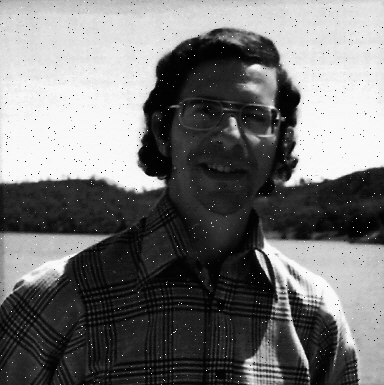
\includegraphics[width=0.5\textwidth]{noised_matloff.jpg}
    \end{center}
  \caption{The image with U(0,1) random noise.}
\end{figure}

\begin{figure}[H]
    \begin{center}
        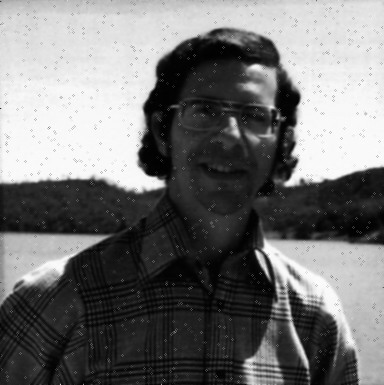
\includegraphics[width=0.5\textwidth]{denoised_matloff.jpg}
    \end{center}
  \caption{After the denoising algorithm is applied.}
\end{figure}

We chose this final image because of its square dimensions, to more closely examine the effect of dimension on the regression coefficients.  We notice that there are definite horizontal patterns (the sky, the mountains in the background), so we assume that the coefficients will be skewed to favor the horizontal pixels, like in the \textit{LaLa Land} picture.  Let's examine (using \textbf{getCoeffs(imgname)} from the appendix):

The regression function for the original image is given by:
\begin{equation}
y = -0.00193 + 0.23920 \cdot N + 0.23914 \cdot S + 0.26273 \cdot E + 0.26322 \cdot W
\end{equation}
We notice that the values of the coefficients are extremely close to one another, and close to being equally weighted in general, but we do have our expected skew towards the horizontal pixels.  This enforces our idea that the patterns have some effect on the skew, because the dimensions of this image do not favor the horizontal or the vertical in terms of the number of available pixels.  In this case, the vast majority of the patterns are broken because of the central figure, which splits the mountain range in the background and the sky with largely vertical patterns in his shirt and shadow, etc.

The regression function for the noisy image is given by:
\begin{equation}
y = -0.00006 + 0.24453 \cdot N + 0.24425 \cdot S + 0.25523 \cdot E + 0.25615 \cdot W
\end{equation}
The random noise behaves as expected, moving the regression coefficients closer to an equal weight algorithm, as the noise acts to destroy any patterns present in the image and make the regression expect nearly equal contribution of each adjacent pixel towards the coloring of the center pixel in the kernel.  This third case enforces our expectations for this pattern of equalizing the coefficients to occur.  In essence, the randomly applied noise skews the averages so far from the original image that it will be impossible to fully restore it.  But we can get close to the original image if we try to reduce this impact, which can be done by extending the kernel further, which is a common practice in image smoothing, as per the description at the beginning of this section.

\newpage
\section{Million Song Dataset}

\subsection{read.csv() vs fread()}

On a speed comparison of \textbf{read.csv} compared to \textbf{fread}, \textbf{fread} is significantly faster to read data than \textbf{read.csv} is. The reason for this is that \textbf{fread} maps the file into memory and then iterates through the file using pointers, while \textbf{read.csv} reads the file into a buffer via a connection, as if it were a character, then attempts to convert the information into a integer or numeric values that could be used in a dataframe \cite{data-table-faq, fread-speed}. The drawbacks to using \textbf{fread} is that it stores the file information into a \textbf{data.table}, which is unable to do certain functions that \textbf{data.frame} is able to do, since it is stored in a different format.

\subsection{The Overloaded Operator of data.table}

The author of \textbf{data.table} overloaded the subscript operator so that it returns a \textbf{data.table} object (instead of a vector like \textbf{data.frame}'s subscript operator does). The \textbf{length} function (for both \textbf{data.table} and \textbf{data.frame}) returns the number of columns, whereas the \textbf{length} function for a vector returns the number of elements. This explains why -- in the example in the project specifications -- \textbf{length(msdf[,1])} returns the number of rows while \textbf{length(msdt[,1])} returns 1.

$\bf{Sources: RDocumentation: https://www.rdocumentation.org/packages/data.table/versions/1.10.4/topics/fread}$

(Find out, again using the Web, why the author made this design choice, and comment.)

\subsection{Difference of Means Analysis}

\subsection{Linear Regression Analysis}

...

Note that this amount of error is actually quite acceptable.  In essence, the number of years our prediction is off by is approximately a range of 10 years, so +- 5 years in either direction.  This is actually rather good if we think about the patterns that are thought to commonly have emerged in music - each decade has its own particular style.  Essentially, using the waveforms and data about a song, we can predict is origin year down to the correct decade.  That is actually quite a remarkable feat - each decade has its own style, and those styles are reflected enough in differences among the data given that we can then narrow the song back down to its decade just by the style as it shows through in audio data.

\subsection{Logistic Regression Analysis}

\subsection{Principal Component Analysis}

\begin{figure}[H]
    \begin{center}
        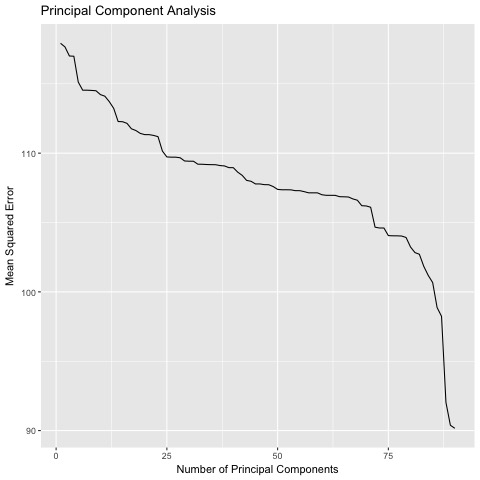
\includegraphics[width=\textwidth]{principalComponent.jpg}
    \end{center}
  \caption{The graph of MSE against number of principal components included.}
\end{figure}

The above image shows the results of performing a version of principal component analysis on the million song data set.  Here, we comprised the set of principal components for the data (the technical details of how that was accomplished are described in Appendix A.4) and used those components to form a new regression function.  Then we performed the regression and calculated the errors as we continued to add principal components.  We see that as we add more principal components to the analysis, the mean-squared error between the predicted years and the actual years for each song is reduced, until it comes down to the level of error that we saw in our original regression analysis.  This is interesting behavior, because we expected to see the function behave slightly differently.

In regression analysis, there is an often arising problem known as "overfitting".  We expect that after a certain number of components taking place in the regression, rather than reduce error as we continue to add new components, the error should actually increase.  This is because once we have too many components, each one may be acting to influence our predictions in ways that the original components never did, and our prediction line is too responsive to the predictor variables.  Then, as the predictor variables have expanded effects, the total prediction ends up far from the real value.  The entire point of principal component analysis is to reduce the number of variables you use in your predictions until you have the optimal number to have the most accurate prediction function.

In our case, the error is continually reduced as we add more variables.  Thus, we can make the conclusion that our prediction function is not "overfit".  Since there are no more principal components to fit into our prediction function, then we know that the optimal prediction is given by using ALL of the principal components in the analysis, giving us the minimal error.

\newpage
\appendix
\section{Code}

\subsection{Problem A - The Code}
% include the code from problem A, then discuss key points from it
\lstinputlisting[language=R]{ProbA.R}
\subsection{Problem A - Code Discussion}
The single largest obstacle to overcome with this program was the runtime.  The process itself behind each function is rather simple: for \textbf{getnonbound} simply finding the greyscale values that correspond to the correct locations, for \textbf{noise} simply generating random U(0,1) noise across an image, and for \textbf{denoise} to run \textbf{getnonbound} and replace the interior pixels by predicted values using the regression of $y$ on $x$.  Each presented unique challenges in vectorization that would prove to significantly reduce the running time of the suite as a whole.

For \textbf{getnonbound}, the largest bottleneck on time was constructing the $x$ matrix.  At its core, it is a simple iteration problem, as shown in the commented out code for that function.  We simply make a count of the current pixel we are trying to get values for, and then go through each pixel in the image by iterating on x and y and getting the neighboring N / S / E / W pixels.  We store this as a matrix and are done.  But, the for loops in R cause significant overhead that can be reduced by vectorizing the arguments as we check pixel locations.  By creating vectors of pixels to examine, we can relate the North pixels to the same x-coordinate and the (y-coordinate$-1$), which is shown through line 32, where the north pixels are all set at the same time, vectorizing access to the greyscale matrix.  The same process is repeated for the South, East, and West pixel locations, and we can construct the final matrix without using any loops.  This \textit{significantly} reduces the runtime of this function, from several or more seconds for a small image (the \textit{LaLa Land} image provided) to milliseconds, and from minutes for large images to only a few seconds.  This does take more memory space though, as we have to create multiple large vectors of simple integer values across the entire width and height of the image.

For \textbf{noise}, the single largest bottleneck on time was applying the random noise to the grayscale matrix of the image.  Generating the random pixels to apply that noise to could also have taken some time if done naively (without the proper use of the sample function or similar processes).  Here we reduce that time bottleneck by vectorizing the X and Y coordinate pairs and binding them together in columns.  This allows us to access each pair as a unit in the matrix and replace it with random noise, all at once as a vector.  As written, the most significant reduction to the running time of this program are the two coordinate checks which validate any incorrect coordinate assignments due to mathematical processes (the ifelse statements).  In addition, setting a large proportion of pixels to be noised in the parameter significantly increases runtime, because the sample must generate many more pixels and the vector arguments for the grayscale matrix and its x- and y-coordinates get much larger.  These large vectors are again the cost of space that we trade off for faster running time.

For \textbf{denoise}, ignoring the runtime of \textbf{getnonbound} the largest time bottleneck was the application of the prediction values to each interior pixel in the image, sped up as in \textbf{getnonbound}'s construction of the $x$ matrix.  It also takes some time to process large vector arguments in the construction of the prediction values.  Both of these are reduced by ensuring everything is vectorized, at the cost of memory space.

\newpage
\subsection{Problem B - The Code}
\lstinputlisting[language=R]{ProbB.R}
\subsection{Problem B - Code Discussion}

...

The \textbf{principalAnalyze} function performs principal component analysis of a sense.  We perform linear regression after finding the principal components to the song data.  The principal components are given as linear combinations of the original V2, ..., V91 data information, so we have to multiply the P matrix through the original data to get a new matrix of the components, with a row for each song.  Then we can perform the regression, each time adding the next most principal component until we are regressing on all components (this is handled in the for loop, which is not-optimal but was as best as we could get the code working for this project).  The PredictorVariables variable stores a copy of strings of all of the columns in the components matrix that we need to perform our regression with, and it is collapsed into a formula to be read by the \textbf{lm()} function which allows us to include one additional variable each time we iterate through the for loop.  Then we calculated the error from these predicted values by principal component using the same method as in the original regression analysis.

\newpage
\section{Distribution of Labor}
\subsection{Joseph Lewis} R coding for Problem A, first and final drafts for the writeup of Problem A and related appendix section, research on image smoothing processes, management of Github repository for project, assistance on Problem B coding and testing for overall coding and write-up details on \textbf{principalAnalyze} function, assistance with optimization and vectorization of all coding, final write-up review and submission.

\subsection{Sean Malloy} Made contributions on the creation of Problem A, such as suggestions and code testing. Edited the term paper/made contributions of the creation of the paper. Made the rough draft for the coding for problem B, and related research on the topics for part B.

\subsection{Aaron Kaloti} Helped work out the approach to Problem A's coding. Wrote certain parts (regarding problem B) of and proofread the term paper. Set up Bibtex. His social security number is 431-52-6319.

\subsection{Luhong Pan} Thanks so much for the wonderful quarter! :)

\subsection{Norm Matloff} We couldn't have done it without you! :)

\newpage
\bibliographystyle{unsrt}
\bibliography{references}

\end{document}